\documentclass[11pt,letterpaper]{article}

% ────────────────────────────────────────────────────────────────
% Packages
% ────────────────────────────────────────────────────────────────
\usepackage[margin=1in]{geometry}
\usepackage{amsmath,amssymb}
\usepackage{booktabs}
\usepackage{enumitem}
\usepackage{hyperref}
\usepackage{xcolor}
\usepackage{listings}
\usepackage{tikz}
\usetikzlibrary{positioning, arrows.meta, fit, calc, shapes.geometric,
                decorations.pathreplacing, backgrounds}
\usepackage{float}
\usepackage{caption}
\usepackage{fancyhdr}
\usepackage{tabularx}
\usepackage{multirow}

\hypersetup{
  colorlinks=true,
  linkcolor=blue!60!black,
  urlcolor=blue!60!black,
  citecolor=blue!60!black
}

% ────────────────────────────────────────────────────────────────
% Listings style
% ────────────────────────────────────────────────────────────────
\lstdefinestyle{sv}{
  language=Verilog,
  basicstyle=\ttfamily\small,
  keywordstyle=\color{blue!70!black}\bfseries,
  commentstyle=\color{green!50!black}\itshape,
  numbers=left,
  numberstyle=\tiny\color{gray},
  frame=single,
  breaklines=true,
  tabsize=2,
  morekeywords={logic,always_ff,always_comb,assign,localparam,typedef,enum,
                unique,case,endcase,generate,genvar,endgenerate,
                module,endmodule,parameter,int,function,endfunction,
                automatic,input,output,begin,end},
  captionpos=b
}

% ────────────────────────────────────────────────────────────────
% Header / Footer
% ────────────────────────────────────────────────────────────────
\pagestyle{fancy}
\fancyhf{}
\lhead{QREM ML-KEM Hardware Accelerator}
\rhead{Memory Connections \& Client Usage}
\cfoot{\thepage}

% ────────────────────────────────────────────────────────────────
\title{%
  \textbf{Memory Bank Connections and Client Usage}\\[0.4em]
  \large QREM Polynomial Memory Subsystem\\[0.4em]
  \normalsize FIPS~203 ML-KEM Hardware Accelerator
}
\author{
  Mavra Muzmmal \and Quardin Lyttle \and Salwan Aldhahab \and
  Jessica Buentipo \and Mai Komar \and Kiet Le
}
\date{York University — Computer Engineering\\[0.3em]\today}

\begin{document}
\maketitle
\thispagestyle{fancy}

% ════════════════════════════════════════════════════════════════
\begin{abstract}
This document explains how the five physical RAM instances in the QREM
polynomial memory subsystem---four polynomial banks and one seed
store---are connected to the three system clients (PAU, HSU, Transcoder)
and the internal wipe FSM. For each client, it describes \emph{what}
data is stored, \emph{why} that client needs it, and \emph{how} the
data flows through the scheduling, bank-mapping, and response-routing
logic.
\end{abstract}

\tableofcontents
\newpage

% ════════════════════════════════════════════════════════════════
\section{Physical Memory Resources}
\label{sec:resources}

The memory subsystem contains exactly \textbf{five RAM instances}
(Figure~\ref{fig:phy}):

\begin{table}[H]
\centering
\caption{Physical RAM inventory.}
\label{tab:rams}
\begin{tabular}{@{}llccl@{}}
\toprule
\textbf{Instance} & \textbf{Module} & \textbf{Width} & \textbf{Depth} &
\textbf{Purpose} \\
\midrule
\texttt{u\_poly\_mem/G\_BANK[0]} & \texttt{poly\_ram\_bank} & 16\,b & 2048 & Poly Bank~0 \\
\texttt{u\_poly\_mem/G\_BANK[1]} & \texttt{poly\_ram\_bank} & 16\,b & 2048 & Poly Bank~1 \\
\texttt{u\_poly\_mem/G\_BANK[2]} & \texttt{poly\_ram\_bank} & 16\,b & 2048 & Poly Bank~2 \\
\texttt{u\_poly\_mem/G\_BANK[3]} & \texttt{poly\_ram\_bank} & 16\,b & 2048 & Poly Bank~3 \\
\texttt{u\_seed\_ram}             & \texttt{seed\_ram}      & 64\,b & 32   & Seed \& Protocol Store \\
\bottomrule
\end{tabular}
\end{table}

\begin{itemize}
  \item Each \textbf{polynomial bank} is a dual-port RAM. The wrapper binds
    generic Port~0 to physical Port~A and generic Port~1 to physical Port~B,
    and either generic port may be a legal read vector or write vector in a
    cycle.
  \item The \textbf{seed RAM} is a lightweight true-dual-port synchronous
    RAM with one HSU-side access port and one Transcoder-side access port.
\end{itemize}

% ════════════════════════════════════════════════════════════════
\section{Connection Topology}
\label{sec:topology}

\begin{figure}[H]
\centering
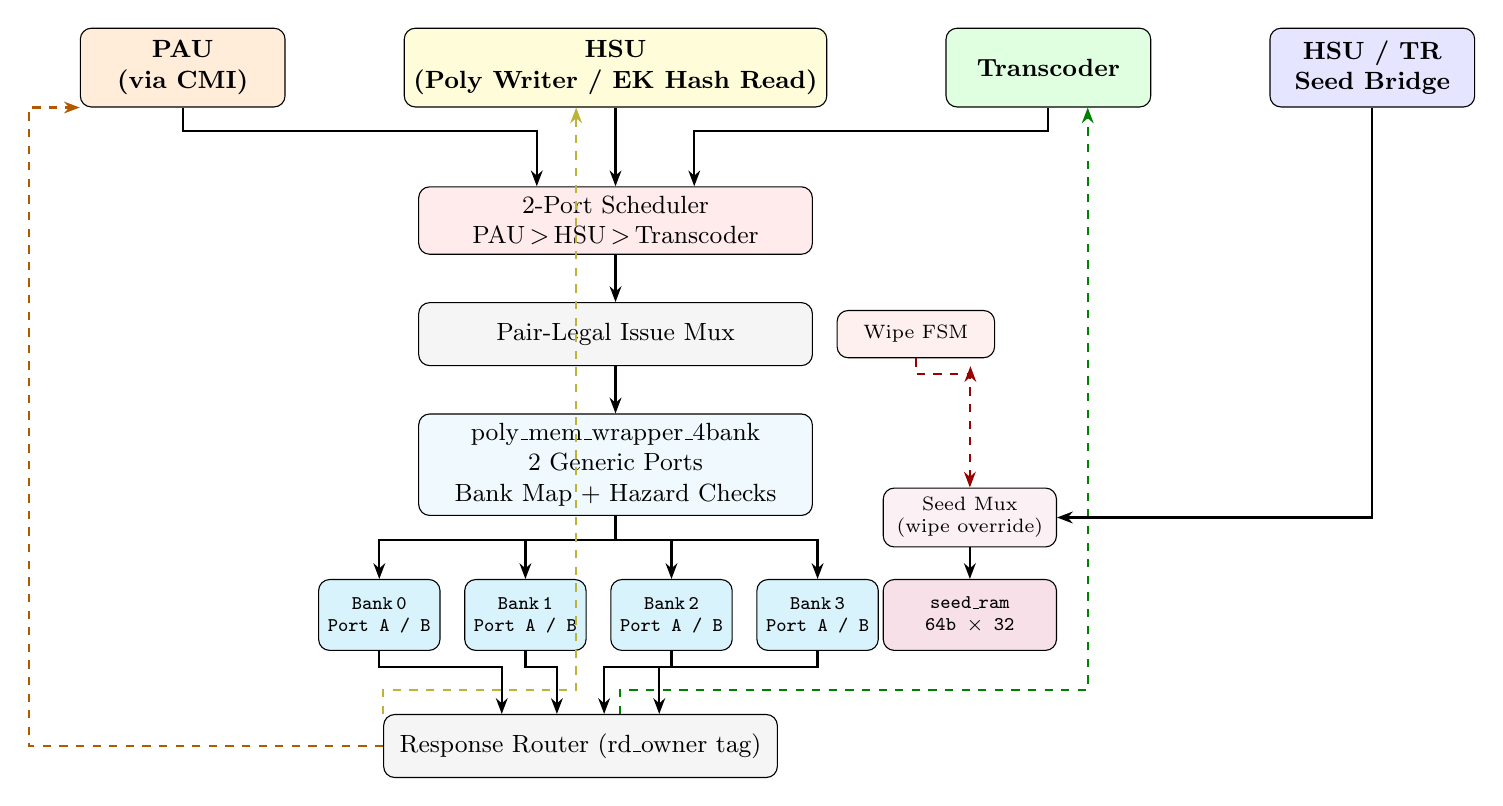
\begin{tikzpicture}[
  client/.style={draw, rounded corners, minimum width=2.6cm,
                 minimum height=1.0cm, font=\small\bfseries, align=center},
  logic/.style={draw, rounded corners, minimum width=3.5cm,
                minimum height=0.8cm, font=\small, align=center,
                fill=gray!8},
  bank/.style={draw, rounded corners, minimum width=1.4cm,
               minimum height=0.9cm, font=\scriptsize\ttfamily,
               align=center, fill=cyan!15},
  seed/.style={draw, rounded corners, minimum width=2.2cm,
               minimum height=0.9cm, font=\scriptsize\ttfamily,
               align=center, fill=purple!12},
  arr/.style={-{Stealth[length=2mm]}, thick},
  darr/.style={-{Stealth[length=2mm]}, thick, dashed},
  node distance=0.5cm
]

% Clients
\node[client, fill=orange!15] (pau) {PAU\\(via CMI)};
\node[client, fill=yellow!15, right=1.5cm of pau] (hsu) {HSU\\(Poly Writer / EK Hash Read)};
\node[client, fill=green!12, right=1.5cm of hsu] (tr) {Transcoder};
\node[client, fill=blue!10, right=1.5cm of tr] (ext) {HSU / TR\\Seed Bridge};

% Scheduler
\node[logic, fill=red!8, minimum width=5cm, below=1.0cm of hsu] (arb)
  {2-Port Scheduler\\PAU\,$>$\,HSU\,$>$\,Transcoder};

% Request mux
\node[logic, minimum width=5cm, below=0.6cm of arb] (mux)
  {Pair-Legal Issue Mux};

% Wrapper
\node[logic, fill=cyan!6, minimum width=5cm, below=0.6cm of mux]
  (wrap) {poly\_mem\_wrapper\_4bank\\2 Generic Ports\\Bank Map + Hazard Checks};

% Banks
\node[bank, below=0.8cm of wrap, xshift=-3cm] (b0) {Bank\,0\\Port A / B};
\node[bank, right=0.3cm of b0] (b1) {Bank\,1\\Port A / B};
\node[bank, right=0.3cm of b1] (b2) {Bank\,2\\Port A / B};
\node[bank, right=0.3cm of b2] (b3) {Bank\,3\\Port A / B};

% Response router
\node[logic, below=0.8cm of b1, xshift=0.7cm, minimum width=5cm] (rsp)
  {Response Router (rd\_owner tag)};

% Seed RAM
\node[seed, below=0.8cm of wrap, xshift=4.5cm] (sram) {seed\_ram\\64b $\times$ 32};

% Seed mux
\node[logic, fill=purple!6, above=0.4cm of sram, minimum width=2.2cm,
      minimum height=0.6cm, font=\scriptsize] (smux) {Seed Mux\\(wipe override)};

% Wipe FSM
\node[logic, fill=red!6, minimum width=2cm, minimum height=0.6cm,
      font=\scriptsize, right=0.3cm of mux] (wipe) {Wipe FSM};

% ── Client → Arbiter ──
\draw[arr] (pau.south) -- ++(0,-0.3) -| ([xshift=-1cm]arb.north);
\draw[arr] (hsu.south) -- (arb.north);
\draw[arr] (tr.south) -- ++(0,-0.3) -| ([xshift=1cm]arb.north);

% ── Arbiter → Mux ──
\draw[arr] (arb.south) -- (mux.north);

% ── Mux → Wrapper ──
\draw[arr] (mux.south) -- (wrap.north);

% ── Wrapper → Banks ──
\draw[arr] (wrap.south) -- ++(0,-0.3) -| (b0.north);
\draw[arr] (wrap.south) -- ++(0,-0.3) -| (b1.north);
\draw[arr] (wrap.south) -- ++(0,-0.3) -| (b2.north);
\draw[arr] (wrap.south) -- ++(0,-0.3) -| (b3.north);

% ── Banks → Response router ──
\draw[arr] (b0.south) -- ++(0,-0.2) -| ([xshift=-1cm]rsp.north);
\draw[arr] (b1.south) -- ++(0,-0.2) -| ([xshift=-0.3cm]rsp.north);
\draw[arr] (b2.south) -- ++(0,-0.2) -| ([xshift=0.3cm]rsp.north);
\draw[arr] (b3.south) -- ++(0,-0.2) -| ([xshift=1cm]rsp.north);

% ── Response router → Clients (dashed back) ──
\draw[darr, orange!70!black] (rsp.west) -- ++(-4.5,0) |- (pau.south west);
\draw[darr, yellow!70!black] (rsp.north west) -- ++(0,0.3) -| ([xshift=-0.5cm]hsu.south);
\draw[darr, green!50!black] ([xshift=0.5cm]rsp.north) -- ++(0,0.3) -| ([xshift=0.5cm]tr.south);

% ── Ext → Seed Mux ──
\draw[arr] (ext.south) |- (smux.east);

% ── Seed Mux → Seed RAM ──
\draw[arr] (smux.south) -- (sram.north);

% ── Wipe → Mux + Seed Mux ──
\draw[darr, red!60!black] (wipe.south) -- ++(0,-0.2) -| ([xshift=2cm]mux.south east);
\draw[darr, red!60!black] (wipe.south) -- ++(0,-0.2) -| (smux.north);

\end{tikzpicture}
\caption{Connection topology. Solid arrows show the request path;
dashed arrows show read-response return and wipe override paths.
All three clients share the same 4 polynomial banks through the internal
2-port scheduler. The seed RAM sits on a separate dual-port path and is
not arbitrated with polynomial traffic.}
\label{fig:phy}
\end{figure}

\subsection{Key Observation: Shared Banks, Not Partitioned}

There is \textbf{no per-client bank partitioning}. All three
clients---PAU, HSU, and Transcoder---share all four polynomial banks
through the same scheduler and wrapper. The subsystem may admit up to two
legal single-sided requests in a cycle; if a client presents a combined
read+write request, it owns both internal ports atomically. PAU may also
own both ports through its primary and auxiliary descriptors when the pair
is legal. Every issued
request is routed through the \emph{same}
\texttt{poly\_mem\_wrapper\_4bank} instance, which applies the same
Memory-side bank-mapping function regardless of which client is requesting.

The seed RAM is on a \textbf{completely separate dual-port path} that
bypasses the polynomial scheduler entirely.

% ════════════════════════════════════════════════════════════════
\section{How a Request Reaches the Banks}
\label{sec:datapath}

The following numbered steps trace a single client request from
initiation to response:

\begin{enumerate}
  \item \textbf{Client asserts request.} The client drives its
    \texttt{*\_req}, \texttt{*\_poly\_id}, read/write indices, and data
    signals.

  \item \textbf{Scheduler resolves priority.} The subsystem chooses the
    highest-priority schedulable request first, then admits a second
    request only if the pair is legal after bank/address analysis.

  \item \textbf{Issue mux selects admitted requests.} Inside
    \texttt{poly\_mem\_subsystem}, combinational issue logic forwards up
    to two admitted client requests to the internal wrapper ports.

  \item \textbf{Wipe mux overrides (if active).} If the wipe FSM is
    active, its internally generated zero-write command replaces the
    client-muxed signals. All client requests are gated off during wipe.

  \item \textbf{Wrapper applies Memory-side bank mapping.} For each of the 4~lanes,
    \texttt{poly\_mem\_wrapper\_4bank} computes:
    \begin{align*}
      \text{bank}[i] &= \texttt{mem\_bank\_idx}(\text{idx}[i]) \\
      \text{addr}[i] &= \texttt{mem\_bank\_addr}(\text{poly\_id},\;\text{idx}[i])
    \end{align*}

  \item \textbf{Conflict check.} The wrapper rejects same-request lane
    conflicts and same-address cross-port hazards. At the top level, the
    scheduler already filters unsafe cross-client pairings before issue.

  \item \textbf{Bank access.} If no conflict:
    \begin{itemize}
      \item \textbf{Reads} $\to$ the admitted generic port drives the
        selected physical RAM port. Data appears one cycle later.
      \item \textbf{Writes} $\to$ the admitted generic port drives
        write-enable, address, and data on the same clock edge.
    \end{itemize}

  \item \textbf{Response routing.} One cycle after accepted reads,
    \texttt{poly\_mem\_subsystem} uses saved owner tags to route up to
    two read responses back to the clients that initiated them. Other
    clients see \texttt{*\_rd\_valid}~$= 0$.
\end{enumerate}

% ════════════════════════════════════════════════════════════════
\section{Per-Client Usage of the Four Polynomial Banks}
\label{sec:clients}

% ────────────────────────────────────────────────────────────
\subsection{PAU (Polynomial Arithmetic Unit) — Highest Priority}

\subsubsection{What It Stores / Accesses}

The PAU reads and writes polynomial coefficients for the following
operations:

\begin{table}[H]
\centering
\caption{PAU operations and their memory access patterns.}
\label{tab:pau_ops}
\begin{tabular}{@{}lllp{5.5cm}@{}}
\toprule
\textbf{Operation} & \textbf{Read} & \textbf{Write} &
\textbf{Access Pattern} \\
\midrule
NTT butterfly & 2~coeffs & 2~coeffs &
  Reads a butterfly pair (indices differ by power-of-2 stride),
  computes the butterfly, writes both results back. \\
INTT butterfly & 2~coeffs & 2~coeffs &
  Inverse direction; same address pattern as NTT. \\
CWM / MAC accumulate & 4+4~coeffs & --- &
  Reads A-row and secret operands, multiplies element-wise,
  and accumulates internally in the PAU MAC register. \\
Row finish / drain & e or acc & 4~coeffs &
  Adds the active error scratch as needed and writes final row
  results back to the selected output slot. \\
ADD drain & 0 & 4~coeffs &
  Write-only phase; drains accumulated results from the AU
  pipeline back to memory. \\
\bottomrule
\end{tabular}
\end{table}

\subsubsection{Why It Needs All 4 Banks}

NTT butterfly pairs at different stages have different stride patterns.
The CMI bit-pair-sum mapping guarantees that every butterfly pair at
every stage maps to \textbf{distinct banks}, so the PAU can read both
butterfly operands in a single cycle without a bank conflict. Without
this property, the NTT would need extra cycles to serialize conflicting
reads, significantly increasing critical-path latency.

\subsubsection{How It Connects}

The PAU does \emph{not} connect directly to the memory subsystem.
Instead, it uses the \textbf{CMI adapter} (\texttt{cmi.sv}), which:

\begin{enumerate}
  \item Receives 4-lane coefficient indices from the PAU controller's
    address generator.
  \item Forwards them as \texttt{pau\_rd\_idx} /
    \texttt{pau\_rd\_lane\_valid} to the memory subsystem.
  \item Receives the 1-cycle-later read response
    (\texttt{pau\_rd\_data}) and presents aligned coefficient values to
    the Arithmetic Unit (AU).
  \item For writes: delays the original read indices through
    configurable \texttt{delay\_n} shift registers (2, 4, 5, or
    9~cycles) so that the write \emph{address} arrives at the memory
    wrapper at the same time as the AU's computed \emph{result data}.
\end{enumerate}

\begin{figure}[H]
\centering
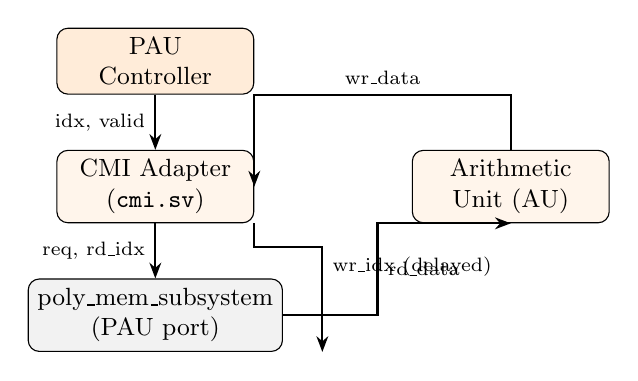
\begin{tikzpicture}[
  block/.style={draw, rounded corners, minimum width=2.5cm,
                minimum height=0.8cm, font=\small, align=center},
  arr/.style={-{Stealth[length=2mm]}, thick},
  node distance=0.7cm
]
\node[block, fill=orange!15] (ctrl) {PAU\\Controller};
\node[block, fill=orange!8, below=of ctrl] (cmi) {CMI Adapter\\(\texttt{cmi.sv})};
\node[block, fill=orange!8, right=2cm of cmi] (au) {Arithmetic\\Unit (AU)};
\node[block, fill=gray!10, below=of cmi] (sub) {poly\_mem\_subsystem\\(PAU port)};

\draw[arr] (ctrl) -- node[left,font=\scriptsize]{idx, valid} (cmi);
\draw[arr] (cmi) -- node[left,font=\scriptsize]{req, rd\_idx} (sub);
\draw[arr] (sub.east) -- ++(1.2,0) |- node[right,font=\scriptsize,pos=0.25]{rd\_data} (au.south);
\draw[arr] (au.north) -- ++(0,0.7) -| node[above,font=\scriptsize,pos=0.25]{wr\_data} (cmi.east);
\draw[arr] (cmi.south east) -- ++(0,-0.3) -| node[below right,font=\scriptsize]{wr\_idx (delayed)} ([xshift=0.5cm]sub.south east);
\end{tikzpicture}
\caption{PAU $\leftrightarrow$ Memory Subsystem connection via CMI.}
\label{fig:pau_conn}
\end{figure}

\subsubsection{Which Polynomial Slots}

The PAU accesses the fixed controller-visible slots depending on the active
ML-KEM operation:

\begin{itemize}
  \item \textbf{NTT/INTT:} Operates in-place on any polynomial slot
    selected by the controller.
  \item \textbf{CWM/MAC:} Reads from two source slots, typically one
    active A row-buffer slot and one $s$ slot, and accumulates internally.
  \item \textbf{ADD drain:} Writes accumulated results from the AU to
    the selected $t$ or work slot.
\end{itemize}

For the corrected KeyGen placement, IDs 0--3 hold $s_0\ldots s_3$ and
are overwritten in place as $\hat{s}$; ID~4 is the active $e_i/\hat{e}_i$
scratch; IDs 5--8 are the active A row buffer; IDs 9--12 hold final
$\hat{t}_0\ldots\hat{t}_3$; IDs 13--31 are generic work slots.

The PAU does \textbf{not} use the seed RAM.

% ────────────────────────────────────────────────────────────
\subsection{HSU (Hash Sampling Unit) — Mid Priority}

\subsubsection{What It Stores / Accesses}

The HSU generates polynomial coefficients through Keccak-based sampling
and writes them into memory:

\begin{table}[H]
\centering
\caption{HSU operations and their memory access patterns.}
\label{tab:hsu_ops}
\begin{tabular}{@{}lllp{5.5cm}@{}}
\toprule
\textbf{Operation} & \textbf{Read} & \textbf{Write} &
\textbf{Access Pattern} \\
\midrule
Sample NTT (rejection) & --- & 4~coeffs/cycle &
  Writes accepted samples sequentially in groups of 4
  via the Poly Stream Writer. \\
Sample CBD & --- & 4~coeffs/cycle &
  Writes centered binomial coefficients for secret/error
  vectors. \\
KG\_HSU\_HASH\_EK & 4~coeffs/cycle & --- &
  Constrained read of final $T0\ldots T3$ slots through the Gearbox
  for ByteEncode12 packing into the HSU hash path. \\
\bottomrule
\end{tabular}
\end{table}

\subsubsection{Why It Needs All 4 Banks}

The HSU writes coefficients in sequential groups of~4. Under the memory-side
bit-pair-sum mapping, consecutive groups of indices
$\{4k, 4k{+}1, 4k{+}2, 4k{+}3\}$ always land in four distinct banks,
so the HSU can sustain one 4-coefficient write per cycle with zero
conflicts.

\subsubsection{How It Connects}

The HSU connects to the \texttt{hsu\_*} port of
\texttt{poly\_mem\_subsystem} through the \textbf{Poly Stream Writer}
bridge (external to this repository). The Poly Stream Writer:

\begin{enumerate}
  \item Receives individual sampled coefficients from the Keccak
    pipeline.
  \item Accumulates them into groups of~4.
  \item Presents a single 4-lane write request to the memory subsystem.
\end{enumerate}

The HSU is \textbf{write-oriented} during sampling and matrix-fill. The
\texttt{hsu\_rd\_*} signals remain at the top-level interface for stability
and for one narrow v0.9 exception: during \texttt{KG\_HSU\_HASH\_EK},
controller/Gearbox glue may assert \texttt{hsu\_hash\_ek\_read\_en} and
read final $T0\ldots T3$ slots only. Non-$T$ slots and HSU mixed read/write
requests still stall cleanly. HSU reads protocol objects such as seeds
through the dedicated \texttt{seed\_*} port instead.

\subsubsection{Which Polynomial Slots}

\begin{itemize}
  \item \textbf{Sample NTT:} Writes the active A row buffer in slots
    5--8. The controller chooses how many of these slots are active for
    $k=2$, $k=3$, or $k=4$.
  \item \textbf{Sample CBD:} Writes secret~$s$ slots 0--3 and the active
    error scratch slot~4 using SHAKE-256 CBD sampling.
  \item \textbf{KG\_HSU\_HASH\_EK:} Reads final $t$ slots 9--12 through a
    Gearbox/read bridge that owns sequencing, ByteEncode12 packing, and
    feeding the HSU hash input. Memory only authorizes and services the
    constrained $T0\ldots T3$ read.
\end{itemize}

\subsubsection{HSU and the Seed RAM}

At the system level, the HSU's Keccak core needs to read the seed
($\rho$ or $\sigma$) to begin hashing. The seed RAM port on
\texttt{poly\_mem\_subsystem} is independent of the polynomial scheduler,
so the system controller can route the HSU's seed reads through the
\texttt{seed\_*} port \textbf{concurrently} with a polynomial bank
access---no arbitration conflict occurs.

% ────────────────────────────────────────────────────────────
\subsection{Transcoder — Lowest Priority}

\subsubsection{What It Stores / Accesses}

The Transcoder converts between the polynomial coefficient
representation and the byte-encoded wire format used in ML-KEM
ciphertexts and public keys:

\begin{table}[H]
\centering
\caption{Transcoder operations and their memory access patterns.}
\label{tab:tr_ops}
\begin{tabular}{@{}lllp{5.5cm}@{}}
\toprule
\textbf{Operation} & \textbf{Read} & \textbf{Write} &
\textbf{Access Pattern} \\
\midrule
ByteEncode & 4~coeffs & --- &
  Reads polynomial coefficients and encodes them into a byte
  stream for transmission. \\
Compress & 4~coeffs & --- &
  Reads coefficients, applies lossy compression
  ($\lceil q/2^d \rfloor$), outputs compressed bytes. \\
ByteDecode & --- & 4~coeffs &
  Receives a byte stream, decodes it into polynomial coefficients,
  and writes them to memory. \\
Decompress & --- & 4~coeffs &
  Receives compressed bytes, reverses the compression, and writes
  recovered coefficients. \\
\bottomrule
\end{tabular}
\end{table}

\subsubsection{Why It Needs All 4 Banks}

The Transcoder accesses coefficients sequentially (index 0, 1, 2, 3,
then 4, 5, 6, 7, \ldots). Under memory-side bank mapping, each group of~4
consecutive indices maps to distinct banks, allowing the Transcoder to
process 4~coefficients per cycle without conflicts.

\subsubsection{How It Connects}

The Transcoder connects directly to the \texttt{tr\_*} port of
\texttt{poly\_mem\_subsystem}. Because it is the lowest-priority
client, it is stalled whenever the PAU or HSU also requests access in
the same cycle. In practice, the Transcoder operates during the
\emph{encoding/decoding phases} of ML-KEM (KeyGen output encoding,
Encaps ciphertext encoding, Decaps ciphertext decoding), which are
typically separate from the NTT/CWM compute phases, so starvation is
rare.

\subsubsection{Which Polynomial Slots}

\begin{itemize}
  \item \textbf{ByteEncode / Compress:} Reads from output~t slots
    (9--12) or controller-selected work slots, producing byte stream output.
  \item \textbf{ByteDecode / Decompress:} Writes received ciphertext
    or public-key bytes into work slots (13--31) or directly into
    controller-selected polynomial slots.
\end{itemize}

The Transcoder does \textbf{not} directly use the seed RAM in typical
operation.

% ════════════════════════════════════════════════════════════════
\section{Seed RAM: Connections and Usage}
\label{sec:seed}

\subsection{Physical Characteristics}

\begin{table}[H]
\centering
\caption{Seed RAM specifications.}
\begin{tabular}{@{}ll@{}}
\toprule
\textbf{Property} & \textbf{Value} \\
\midrule
Module   & \texttt{seed\_ram} \\
Width    & 64 bits \\
Depth    & 32 entries \\
Ports    & True dual-port (HSU + Transcoder) \\
Latency  & 1 cycle (synchronous read) \\
\bottomrule
\end{tabular}
\end{table}

\subsection{Connection Path}

The seed RAM has two independent physical ports on
\texttt{poly\_mem\_subsystem}:

\begin{itemize}
  \item HSU-side: \texttt{hsu\_seed\_req}, \texttt{hsu\_seed\_we},
    \texttt{hsu\_seed\_addr}, \texttt{hsu\_seed\_wdata},
    \texttt{hsu\_seed\_ready}, \texttt{hsu\_seed\_rvalid},
    \texttt{hsu\_seed\_rdata}
  \item Transcoder-side: \texttt{tr\_seed\_req}, \texttt{tr\_seed\_we},
    \texttt{tr\_seed\_addr}, \texttt{tr\_seed\_wdata},
    \texttt{tr\_seed\_ready}, \texttt{tr\_seed\_rvalid},
    \texttt{tr\_seed\_rdata}
\end{itemize}

These ports are \textbf{completely independent} of the PAU/HSU/Transcoder
polynomial scheduler. They can be used \emph{concurrently} with polynomial-bank
traffic.

\subsection{Who Drives the Seed Port?}

The memory subsystem does not enforce semantic ownership. The physical seed
ports are passive RAM interfaces; the system-level integration decides how
bridges and the Main Controller use them. In the QREM architecture:

\begin{table}[H]
\centering
\caption{Seed RAM users in the QREM system.}
\label{tab:seed_users}
\begin{tabular}{@{}lp{8cm}@{}}
\toprule
\textbf{Module} & \textbf{Usage} \\
\midrule
\textbf{HSU (Keccak Core)} &
  Reads the 256-bit seed ($\sigma$ or $\rho$) from the seed RAM and
  feeds it to the SHAKE/SHA3 core for hash-based sampling. This is the
  primary seed consumer. \\
\textbf{Transcoder} &
  Reads or writes protocol values such as $H(ek)$, shared-secret staging,
  or temporary metadata through its dedicated seed-side port. \\
\textbf{System Controller} &
  Writes the initial seed value (from the random number generator or
  received key material) into the seed RAM at the start of each
  KeyGen/Encaps/Decaps operation. \\
\bottomrule
\end{tabular}
\end{table}

\subsection{Bridge-Facing Seed ID + Beat Contract}

Above Memory, the cleaner abstraction is:

\begin{itemize}
  \item \texttt{seed\_id}: semantic object selector such as
    \texttt{SEED\_ID\_RHO}, \texttt{SEED\_ID\_SIGMA}, or
    \texttt{SEED\_ID\_HEK}
  \item \texttt{seed\_idx}: beat offset inside the selected object
\end{itemize}

The physical Seed Store remains address-based. A bridge computes:

\[
  \texttt{seed\_addr = seed\_base\_addr(seed\_id) + seed\_idx}
\]

This keeps Memory simple while reducing magic-address burden on HSU and
Transcoder designers.

\subsection{Seed RAM vs.\ Polynomial Banks: Key Differences}

\begin{table}[H]
\centering
\caption{Comparison between polynomial banks and seed RAM.}
\label{tab:compare}
\begin{tabular}{@{}lll@{}}
\toprule
& \textbf{Polynomial Banks (×4)} & \textbf{Seed RAM (×1)} \\
\midrule
Module       & \texttt{poly\_ram\_bank}     & \texttt{seed\_ram} \\
Width        & 16 bits                       & 64 bits \\
Depth        & 2048 entries each             & 32 entries \\
Ports        & Dual-port (physical A/B under 2-port scheduler) & Dual-port (HSU + Transcoder) \\
Bank mapping & Memory-side bit-pair-sum     & Direct address \\
Arbitrated   & Yes (PAU$>$HSU$>$Transcoder)  & No (independent port) \\
Data stored  & Polynomial coefficients       & Seeds, hash state,
               protocol metadata \\
Wipe phase   & \texttt{WIPE\_POLY} (2048 cy) & \texttt{WIPE\_SEED} (32 cy) \\
\bottomrule
\end{tabular}
\end{table}

\subsection{Seed RAM During Wipe}

When the security wipe FSM reaches the \texttt{WIPE\_SEED} state:

\begin{enumerate}
  \item The wipe FSM overrides \texttt{seed\_we\_mux},
    \texttt{seed\_addr\_mux}, and \texttt{seed\_wdata\_mux} with
    internally generated zero-write commands.
  \item It iterates through all 32~addresses, writing 64'h0 to each.
  \item \texttt{seed\_ready} is deasserted, blocking any external
    access during wipe.
\end{enumerate}

% ════════════════════════════════════════════════════════════════
\section{Wipe FSM: Its Use of Both Memories}
\label{sec:wipe}

The wipe FSM is an internal client of ``last resort''---it has
absolute priority over all three external clients because it gates
their requests off entirely.

\begin{table}[H]
\centering
\caption{Wipe FSM access to each memory resource.}
\label{tab:wipe_access}
\begin{tabular}{@{}llll@{}}
\toprule
\textbf{Phase} & \textbf{Target} & \textbf{Access Type} &
\textbf{Cycles} \\
\midrule
\texttt{WIPE\_POLY} & Banks 0--3 &
  4-lane write (all zeroes) via one generic port &
  $32 \times 64 = 2048$ \\
\texttt{WIPE\_SEED} & Seed RAM &
  Single-word write (zero) &
  32 \\
\texttt{WIPE\_DONE} & None & Signal completion & 1 \\
\midrule
\multicolumn{3}{@{}l}{\textbf{Total}} & \textbf{2081 cycles} \\
\bottomrule
\end{tabular}
\end{table}

During \texttt{WIPE\_POLY}, the FSM writes indices
$\{4r, 4r{+}1, 4r{+}2, 4r{+}3\}$ for each row~$r$. Under memory-side bank mapping,
these four indices always map to four distinct banks, so all four
selected-port write-enables fire simultaneously with no conflict.

% ════════════════════════════════════════════════════════════════
\section{Summary: Complete Access Map}
\label{sec:summary}

\begin{table}[H]
\centering
\caption{Complete access map: which client uses which memory, and how.}
\label{tab:access_map}
\begin{tabularx}{\textwidth}{@{}l c c c c X@{}}
\toprule
& \textbf{Bank 0} & \textbf{Bank 1} & \textbf{Bank 2} &
\textbf{Bank 3} & \textbf{Seed RAM} \\
\midrule
\textbf{PAU} &
\multicolumn{4}{c}{R/W via scheduler (highest priority; PAU-side CMI external)} &
--- \\
\textbf{HSU} &
\multicolumn{4}{c}{W via scheduler; constrained T-slot R during KG\_HSU\_HASH\_EK} &
R/W (dedicated seed-side port) \\
\textbf{Transcoder} &
\multicolumn{4}{c}{R/W via scheduler (lowest priority)} &
R/W (dedicated seed-side port) \\
\textbf{Controller} &
--- & --- & --- & --- &
W via seed bridge / internal control path \\
\textbf{Wipe FSM} &
\multicolumn{4}{c}{W (zeroes all slots; absolute priority via gating)} &
W (zeroes all entries) \\
\bottomrule
\end{tabularx}
\end{table}

\bigskip

\noindent\textbf{Key takeaways:}
\begin{itemize}
  \item The four polynomial banks are a \textbf{shared resource}. No
    bank is ``owned'' by any client---every client's indices pass through
    the same Memory-side bank-mapping function, and the bank each coefficient
    lands in depends solely on the coefficient index, not on which
    client issued the request.
  \item The seed RAM is \textbf{not} part of the polynomial bank array.
    It is a separate, independent dual-port memory with no polynomial-bank
    scheduler involvement.
  \item The polynomial subsystem supports up to two \textbf{legal issued
    requests} per cycle. They may be read/read, write/write, or read/write
    when safe, while a combined read+write request owns both internal ports
    atomically.
  \item The wipe FSM is the only entity that accesses \textbf{both}
    memory types, and it does so sequentially (polynomial banks first,
    then seed RAM).
\end{itemize}

\end{document}
